\documentclass[25pt, portrait]{tikzposter}
%\usepackage{authblk}
\usepackage{tikz}
\tikzposterlatexaffectionproofoff
\usepackage{adjustbox}
\usepackage{textcomp}
\usepackage{multicol}

\usepackage{cite}
\usepackage{booktabs}
\usepackage{bbding}
\usepackage{array}
\usepackage{graphicx}
\usepackage{comment}
\usepackage{subfigure}
\usepackage{enumerate}
\usepackage{epstopdf}
\usepackage{epsfig}
\usepackage{flushend}
\usepackage{tabularx}
\usepackage{textcomp}
\usepackage{enumitem}
\usepackage{amssymb}
\usepackage{amsmath}
\usepackage{amsthm}
\usepackage[english]{babel}
\usepackage{blindtext}	
\usepackage{dsfont}
\usepackage{url}
\usepackage{caption}
\def\UrlBreaks{\do\/\do-}
\usepackage{multirow}

\newcommand{\ie}{{\em i.e.}}
\newcommand{\eg}{{\em e.g.}}
\newcommand{\et}{{\em et al.}}
\newcommand{\st}{{\em s.t.}}

% \usepackage{amssymb}
\usetikzlibrary{shapes, arrows}
\usetheme{Default}

\geometry{paperwidth=100cm, paperheight= 100cm}   %set by yourself
\makeatletter
\setlength{\TP@visibletextwidth}{\textwidth-2\TP@innermargin}
\setlength{\TP@visibletextheight}{\textheight-2\TP@innermargin}
\makeatother

\title{\vspace{-1cm} \parbox{.8\textwidth}{\centering Unlocking the Value of Privacy: Trading Aggregate Statistics over Private Correlated Data}}
\author{\vspace{.2cm} Chaoyue~Niu, Zhenzhe~Zheng, Fan~Wu, Shaojie~Tang$^\dag$, Xiaofeng~Gao, and Guihai~Chen \vspace{-.6cm}}
\institute{  Shanghai Key Laboratory of Scalable Computing and Systems, Shanghai~Jiao~Tong~University, China\\
	         $^\dag$Department of Information Systems, University of Texas at Dallas, USA\\ \vspace{.2cm}
	         Email:\{rvince, zhengzhenzhe, wu-fan\}@sjtu.edu.cn; tangshaojie@gmail.com; \{gao-xf, gchen\}@cs.sjtu.edu.cn
\vspace{-.4cm}
}


\makeatletter
\renewenvironment{tikzfigure}[1][]{
  \def \rememberparameter{#1}
  \vspace{10pt}
  \refstepcounter{figurecounter}
  \begin{center}
  }{
    \ifx\rememberparameter\@empty
    \else %nothing
    \\[10pt]
    {\large Fig.~\thefigurecounter.~\rememberparameter}
    \\[15pt]
    \fi
  \end{center}
}
\makeatother

\makeatletter
\newcounter{tablecounter}
\newenvironment{tikztable}[1][]{
  \def \rememberparameter{#1}
  \vspace{10pt}
  \refstepcounter{tablecounter}
  \begin{center}
  }{
    \ifx\rememberparameter\@empty
    \else
    %\\[10pt]
    {\large Table~\uppercase\expandafter{\romannumeral\thetablecounter}. \sc \rememberparameter}
    %\\[15pt]
    \fi
  \end{center}
}
\makeatother


\begin{document}
  \maketitle[width=0.9\textwidth]
  \begin{columns}
    \column{0.26}
    \block{\sc Introduction}
    {
    	\begin{center}
    		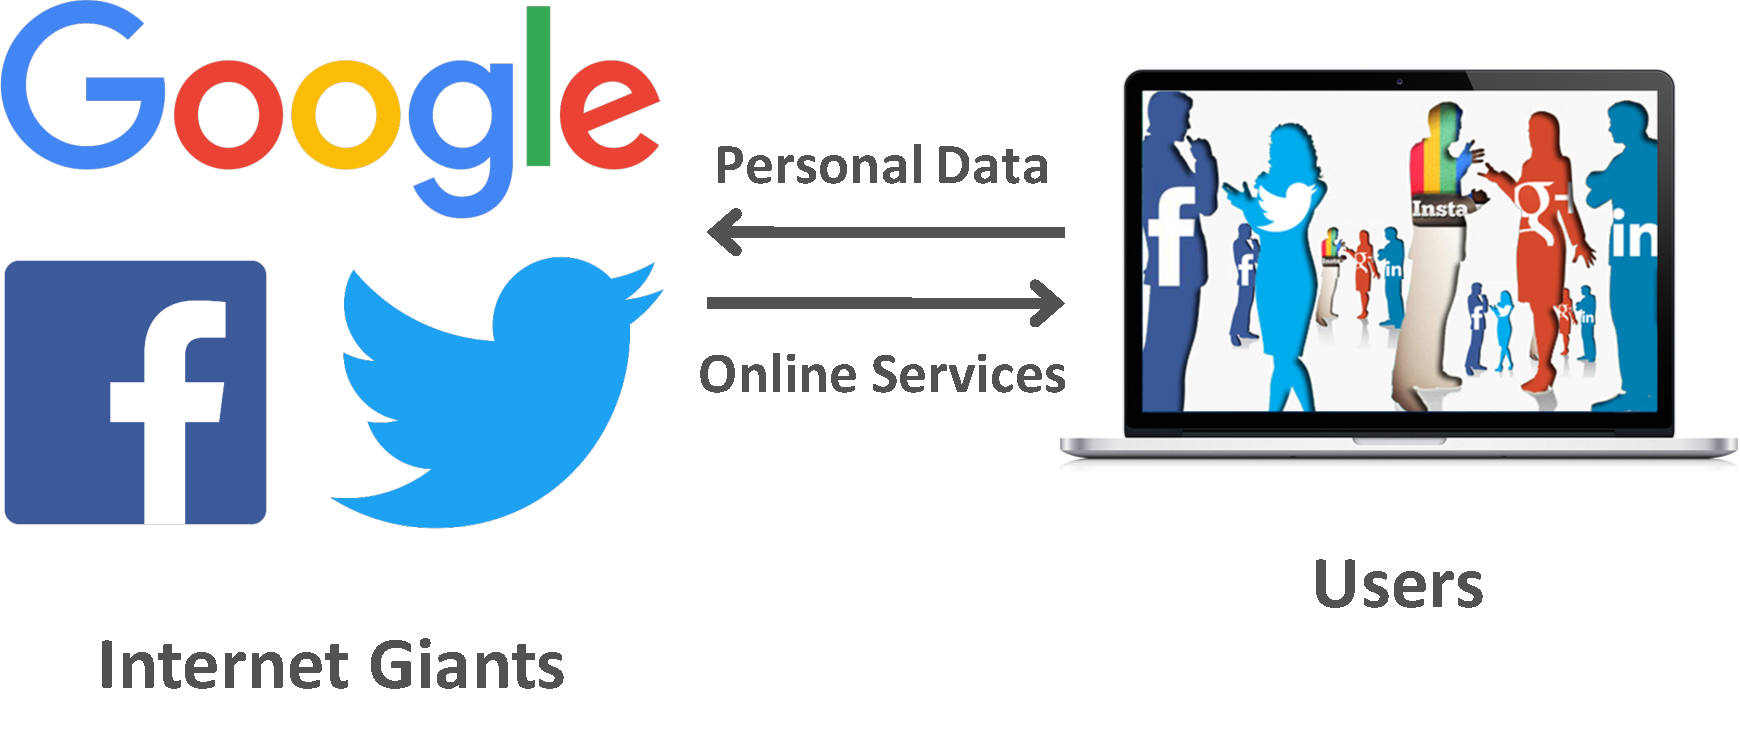
\includegraphics[width=.92\colwidth]{images/data-circulation1}
    	\end{center}
       \vspace{-.4cm}
       \begin{tikzfigure}[Private Data Circulations in Real Life.]
           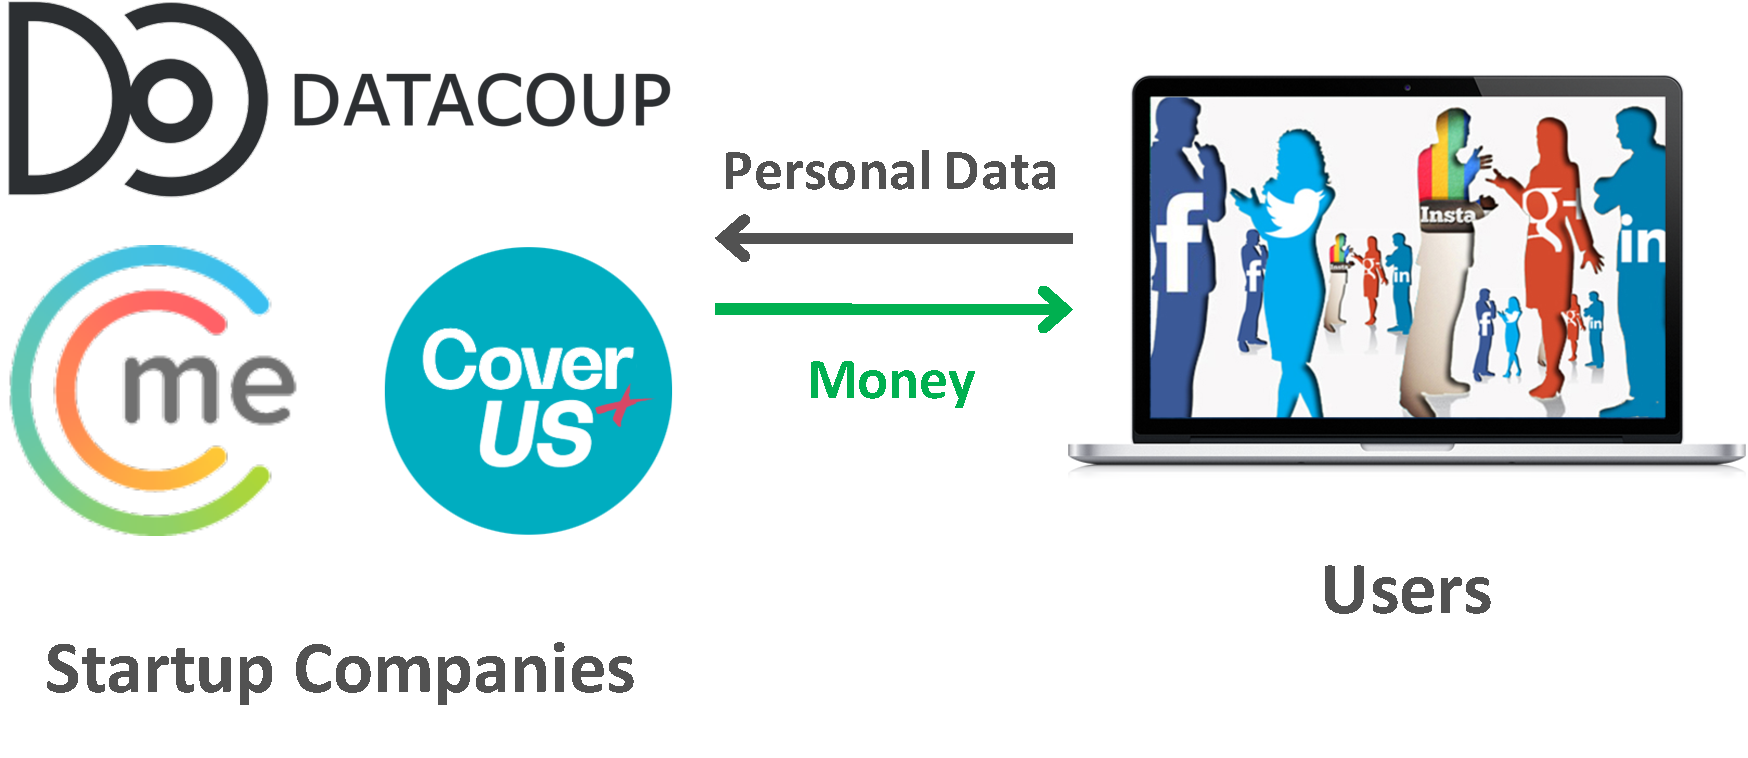
\includegraphics[width=.92\colwidth]{images/data-circulation2}
       \end{tikzfigure}

       \vspace{0.1cm}
       \begin{center}
       	  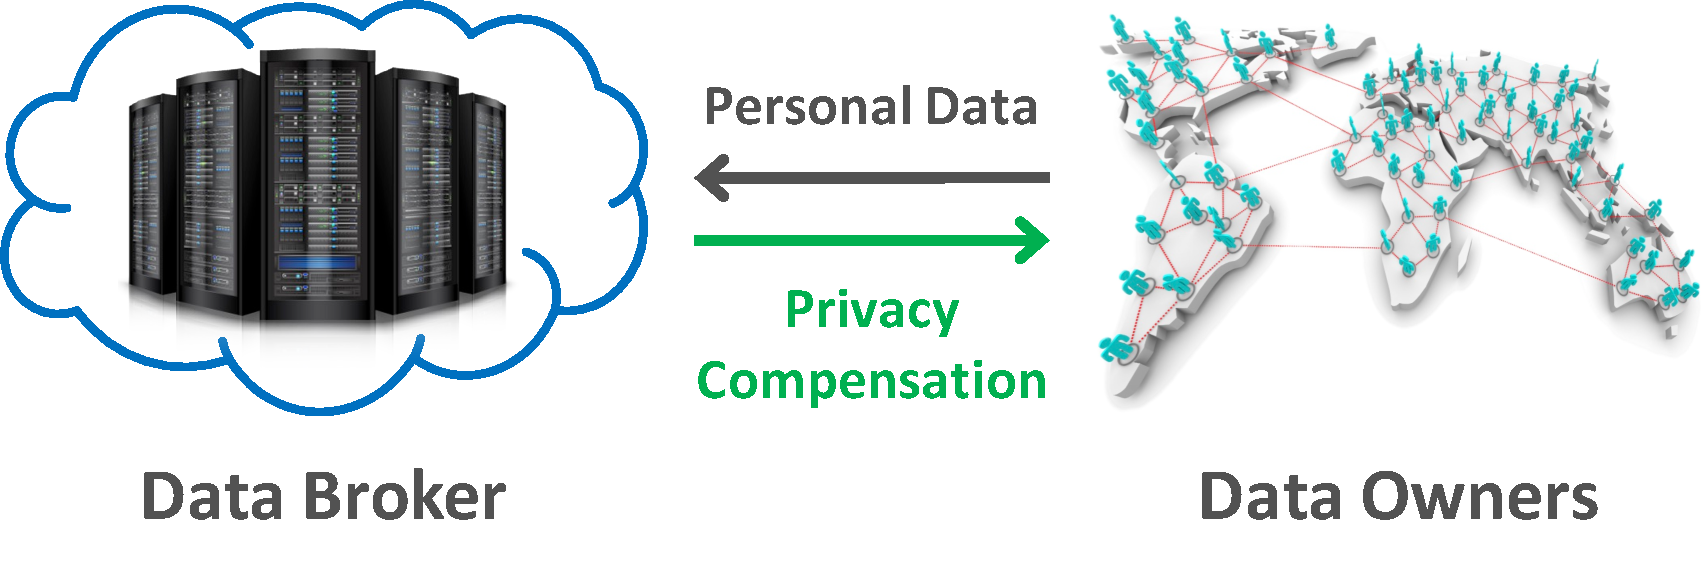
\includegraphics[width=.92\colwidth]{images/data-acq}
       \end{center}
       \vspace{-.7cm}
       \begin{tikzfigure}[A General System Model of Data Markets.]
       	  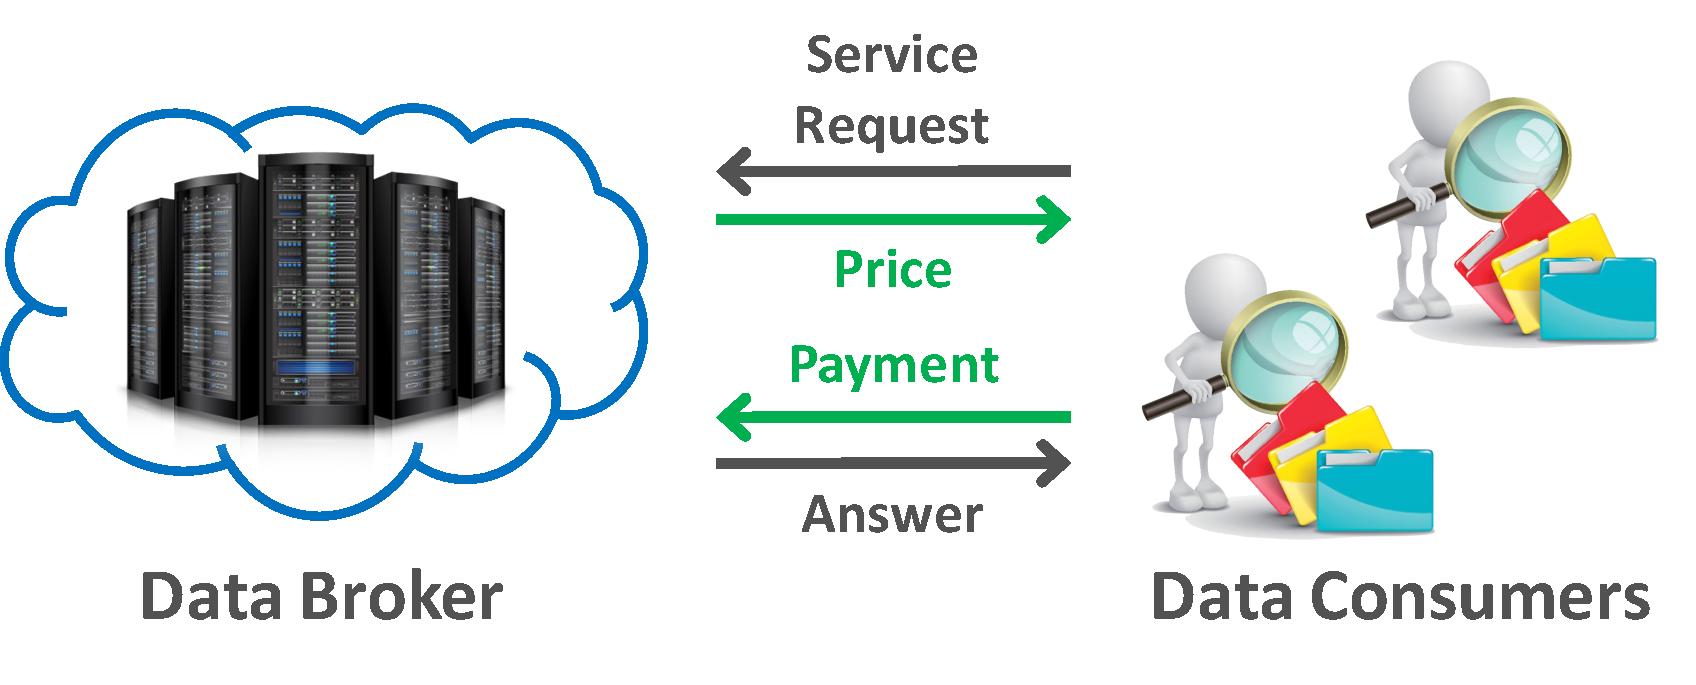
\includegraphics[width=.92\colwidth]{images/data-trading2}
       \end{tikzfigure}

       \vspace{-.8cm}
       \begin{tikzfigure}[Service Requests from Data Consumers.]
       	  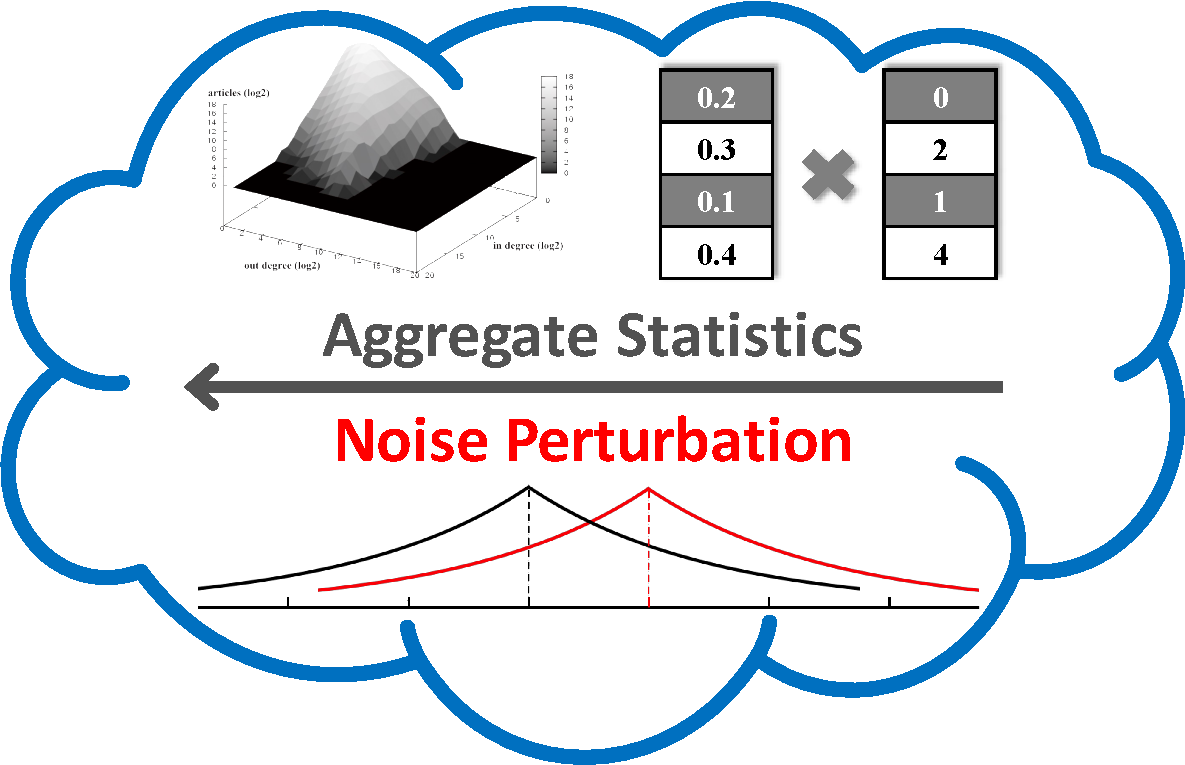
\includegraphics[width=.92\colwidth]{images/service-request}
       \end{tikzfigure}

      \vspace{-.6cm}
       \begin{tikzfigure}[The Elementary Dot Product Operation Underlying Common Aggregate Statistics.]
       	  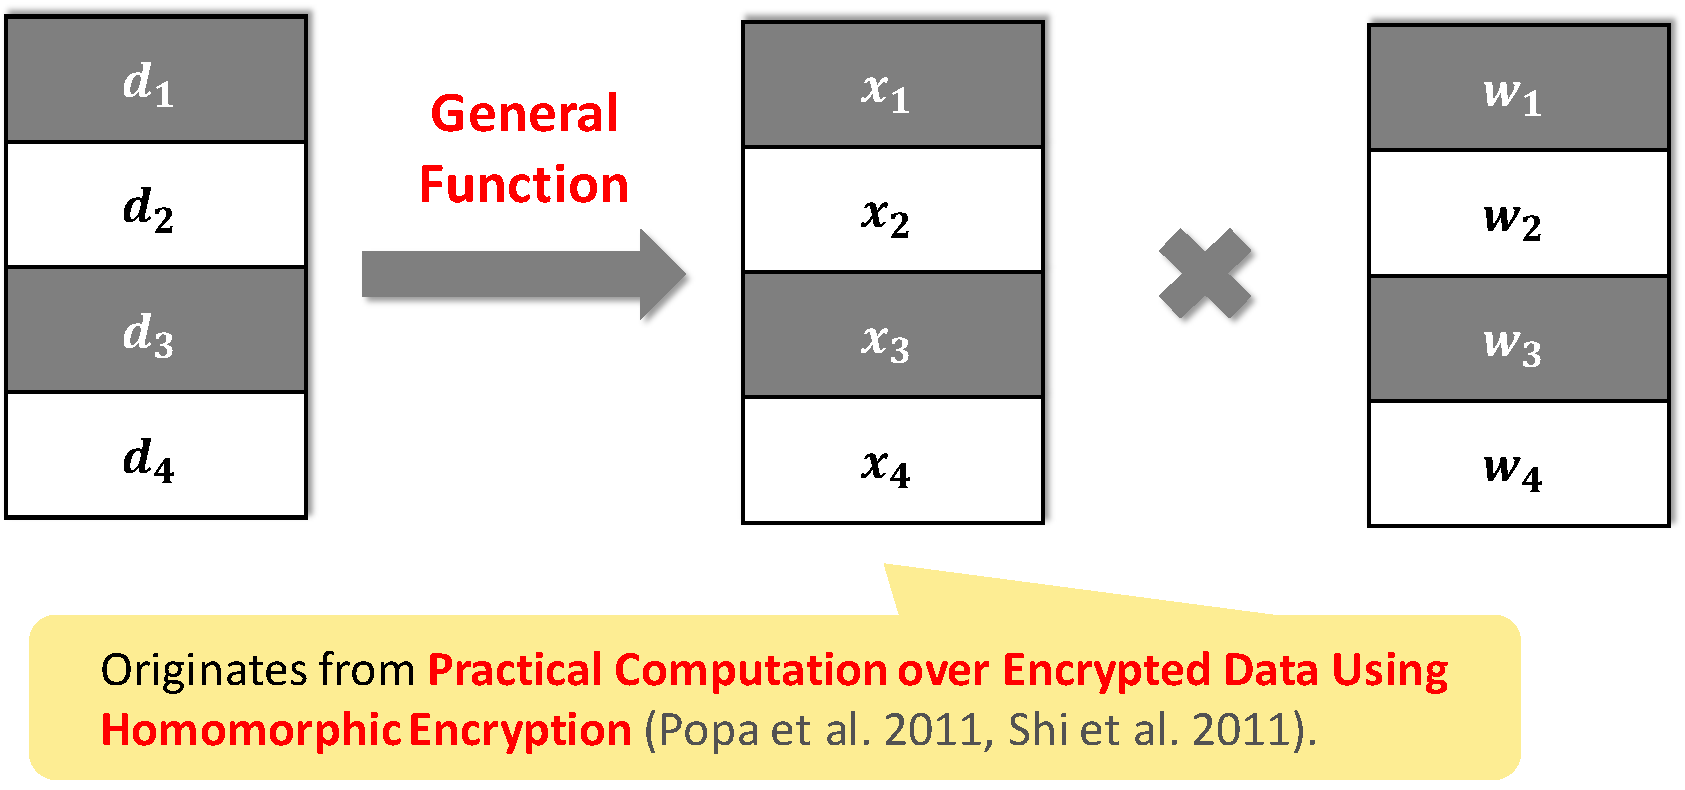
\includegraphics[width=.92\colwidth]{images/dot-product}
       \end{tikzfigure}
       \vspace{-.4cm}
    }
    \column{0.32}
	\block{\sc Service Pricing}
    {
    	\vspace{-.4cm}
       \begin{tikzfigure}[Service Determinacy and Arbitrage Freeness.]
          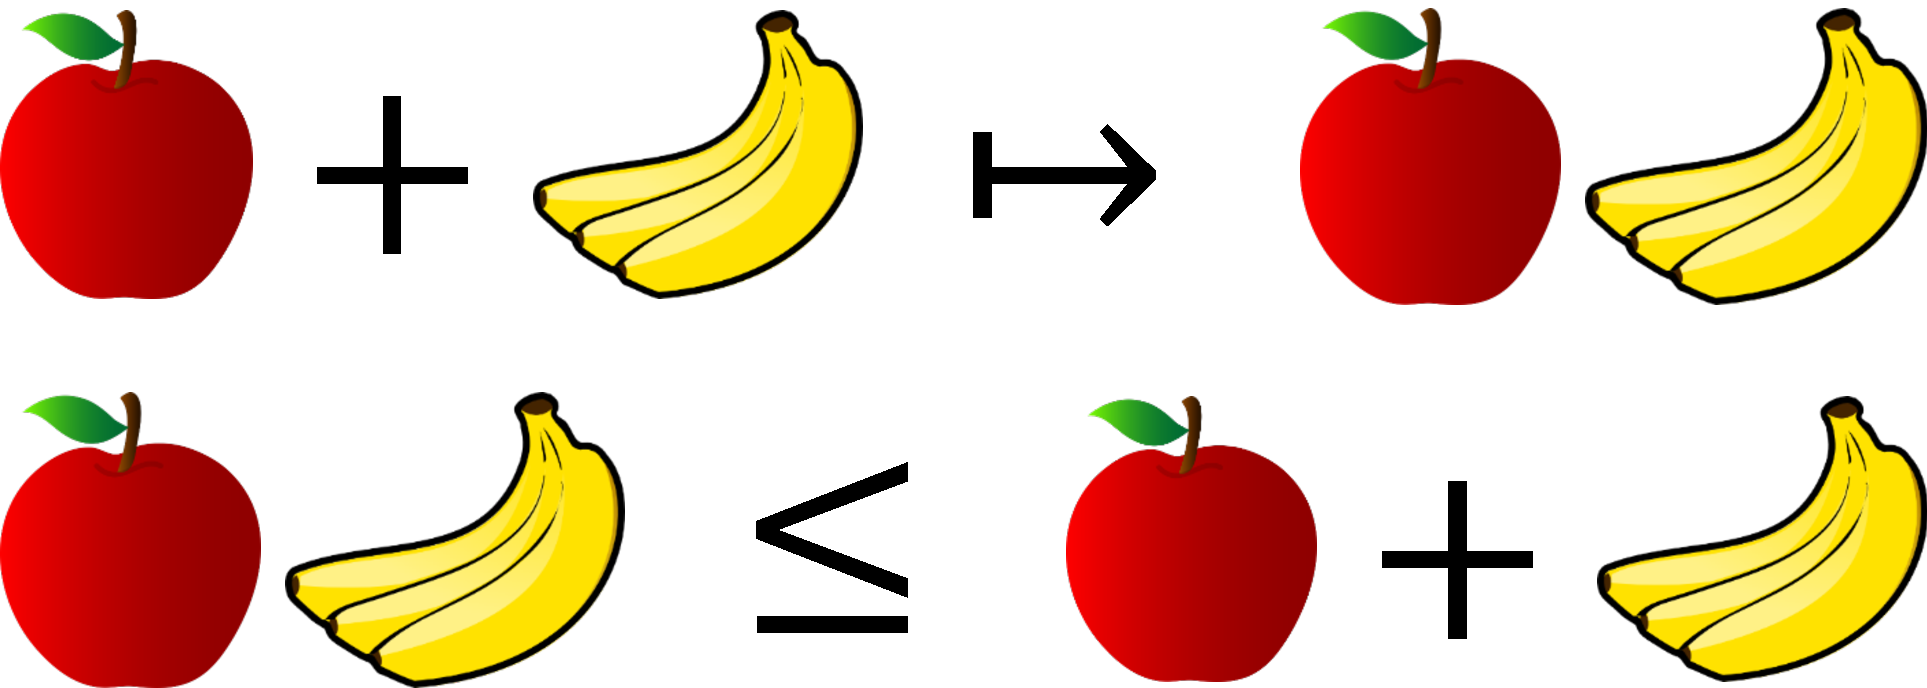
\includegraphics[width=0.81\colwidth]{images/apple}
          \vspace{.4cm}
       \end{tikzfigure}
       \vspace{.3cm}
      \innerblock{Incorporating Variance of Noise}
      {
      	   \coloredbox[bgcolor=white,fgcolor=black,framecolor=gray]
      	   {
      	   	\textsc{Motivating Example.} Get $(\mathbf{w}, v)$ with a lower price?
      	   	\begin{align*}
                \left\{\left(\mathbf{w}, v_1\right) \ldots \left(\mathbf{w}, v_m\right)\right\} \mapsto \left(m\mathbf{w}, \sum_{j=1}^{m} v_j\right) \mapsto \left(\mathbf{w}, \frac{1}{m^2}\sum_{j=1}^{m}v_j\right).
      	   	\end{align*}
           }
           \vspace{.1cm}
         	\coloredbox[bgcolor=white,fgcolor=black,framecolor=gray]
         	{
               \textsc{Theorem 1.} For any arbitrage-free pricing function $\pi(\mathbf{w}, v)$, with two independent parts: the weight vector $\mathbf{w}$ and the variance of noise $v$, it {\bf\color{red}cannot decrease faster than $1/v$}.
         	}
      }
      \vspace{.3cm}
      \innerblock{Incorporating Weight Vector}
      {
      	    \coloredbox[bgcolor=white,fgcolor=black,framecolor=gray]
      	    {
              \textsc{Theorem 2 (Basic Arbitrage-free Pricing Functions).} Let {\bf\color{red}$\pi(\mathbf{w}, v) = g(\mathbf{w})^2/v$} be the pricing function for some positive function $g(\mathbf{w})$ that only depends on $\mathbf{w}$. Then, {\bf\color{red}$\pi(\mathbf{w}, v)$ } is {\bf\color{red}arbitrage free iff $g(\mathbf{w})$} is a {\bf\color{red}semi-norm}.
      	    }
           \vspace{.1cm}
           \coloredbox[bgcolor=white,fgcolor=black,framecolor=gray]
           {
              \textsc{Theorem 3 (Composite Arbitrage-free Pricing Functions).} Let $\Gamma: \mathbb{R}^{\phi} \rightarrow \mathbb{R}$ be a {\bf\color{red}nondecreasing} and {\bf\color{red}subadditive} function. For any set of arbitrage-free pricing functions $\{\pi_1(S), \ldots, \pi_{\phi}(S)\}$, the composite pricing function $\pi(S) = \Gamma(\pi_1(S), \ldots, \pi_{\phi}(S))$ is also arbitrage free.
           }
       }
    }
	%\note[targetoffsetx=9.8cm, targetoffsety=-11.4cm, width=14.4cm,innersep=0.2cm,roundedcorners=0]{BGN}
    \block{\sc Privacy Compensation}
    {
      	\coloredbox[bgcolor=white,fgcolor=black,framecolor=gray]
      	{
      		\textsc{Definition 1 (Individual Privacy Loss).} The privacy loss of the data owner $i$ is defined as:
      		\begin{align*}
              \epsilon_i(\mathcal{M}) = \sup_{\mathbf{x}, O}\left\vert \log\frac{P\left(\mathcal{M}\left(\mathbf{x}\left(L, R\right)\right) = O\right)}{P\left(\mathcal{M}\left(\mathbf{x}^{(i)}\left(L, R\right)\right) = O\right)}\right\vert.
      		\end{align*}
      		Here, $\mathbf{x}\left(L, R\right)$ and $\mathbf{x}^{(i)}\left(L, R\right)$ {\bf\color{red}initially} differ in $x_i$.
      		%where $\mathbf{x}$ ranges over all possible database instances, and $O$ ranges over all possible outputs.
      	}

       \begin{tikzfigure}[Bottom-up Design of Privacy Compensation.]
          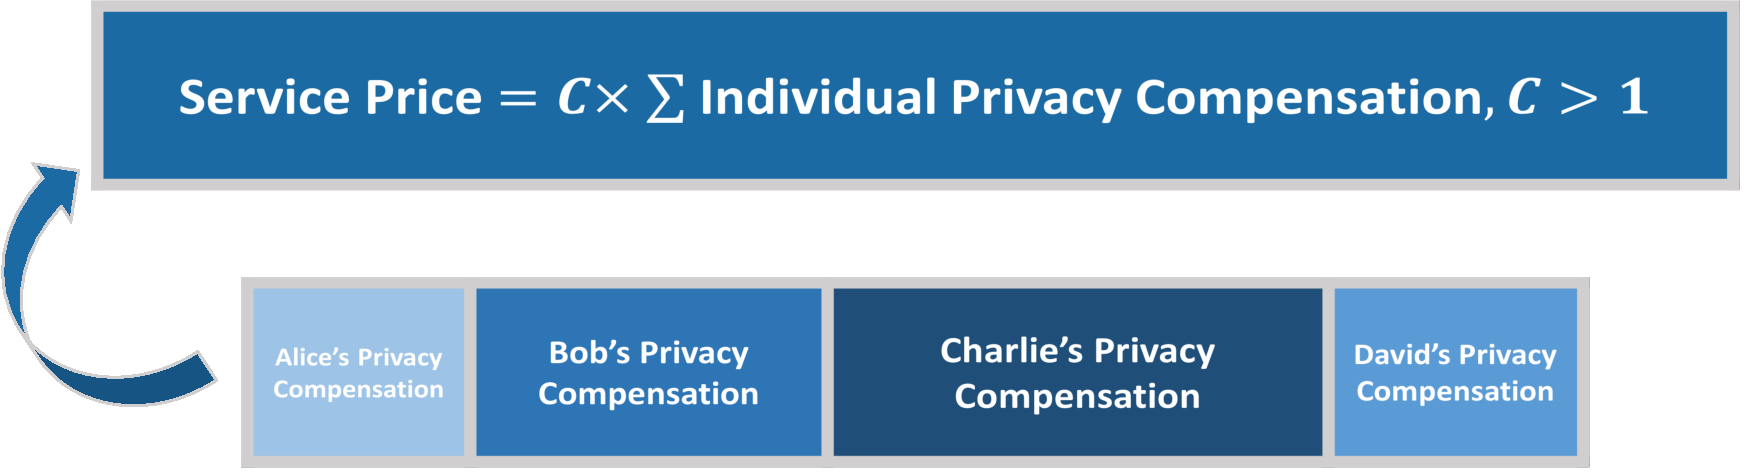
\includegraphics[width=0.85\colwidth]{images/bottom-up.pdf}
       \end{tikzfigure}
        \vspace{-.6cm}
       \begin{tikzfigure}[Top-down Design of Privacy Compensation.]
       	  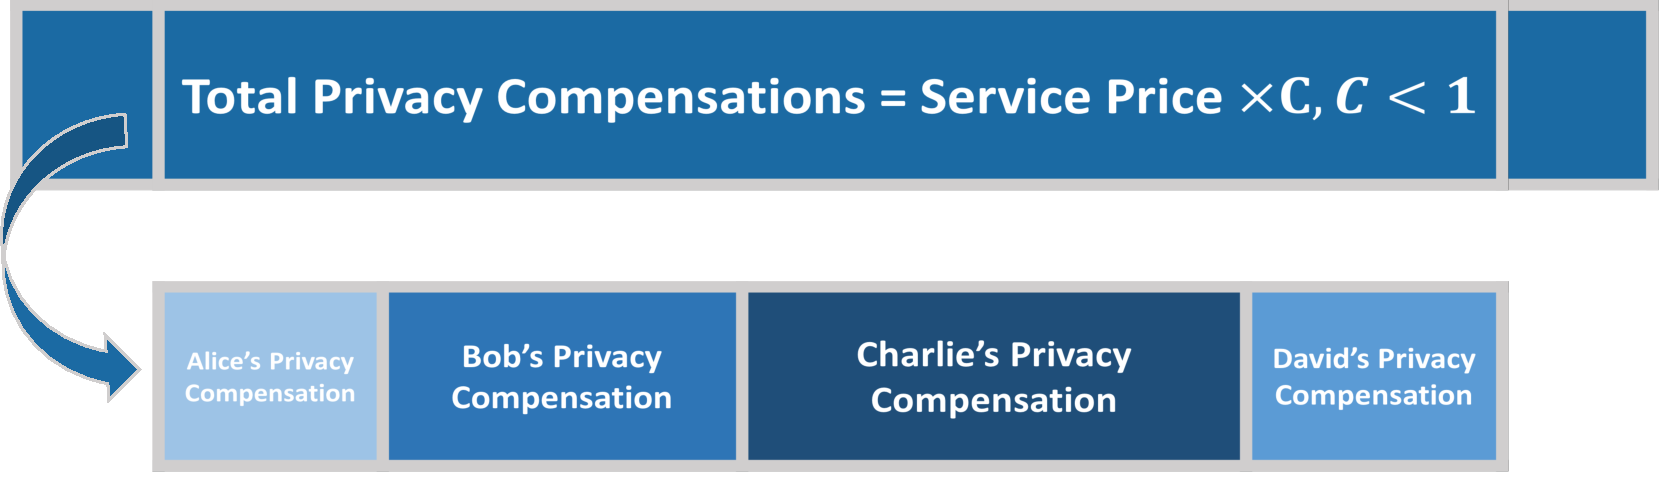
\includegraphics[width=0.85\colwidth]{images/top-down.pdf}
       \end{tikzfigure}
      \vspace{-.6cm}
    }
   \column{0.42}
   %\block[titleoffsety=3cm,bodyoffsety=3cm,titleoffsetx=-.182\colwidth,titlewidthscale=.62,]{Evaluation Results}{
   \block{\sc Evaluation Results}
   {
  	\vspace{-.2cm}
  	\coloredbox[bgcolor=white,fgcolor=black,framecolor=gray]
  	{
  	   %\textsc{Four Real-world Datasets.}
  	   \begin{itemize}[labelsep=\fontdimen2\font]
         \item {\bf\color{red} MovieLens} 1M dataset: {\bf\color{red} 1,000,209 ratings} of approximately {\bf\color{red} 3900 movies} made by {\bf\color{red} 6040 users}; {\bf\color{red} Displayed ratings} as {\bf\color{red} target variables} in supervised learning.
  		 \item 2009 {\bf\color{red} Residential Energy Consumption Survey} (RECS) dataset: Released by U.S. {\bf\color{red} EIA} in Jan. 2013; Diverse energy usages in {\bf\color{red} 12,083 U.S. homes}.
         \item Two social network datasets from {\bf\color{red} Stanford Network Analysis Platform} (SNAP): ego-Twitter: {\bf\color{red} 81,306 nodes} and {\bf\color{red} 1,768,149 edges} from {\bf\color{red} Twitter}; ego-Google+: {\bf\color{red} 107,614 nodes} and {\bf\color{red} 13,673,453 edges} from {\bf\color{red} Google+}.
  	    \end{itemize}
      }
     \vspace{-.2cm}
  	  \begin{tikzfigure}[Privacy vs. Utility and Arbitrage Freeness in Weighted Sum. ]
  		  \label{fig:sp:weighted:sum}
  		  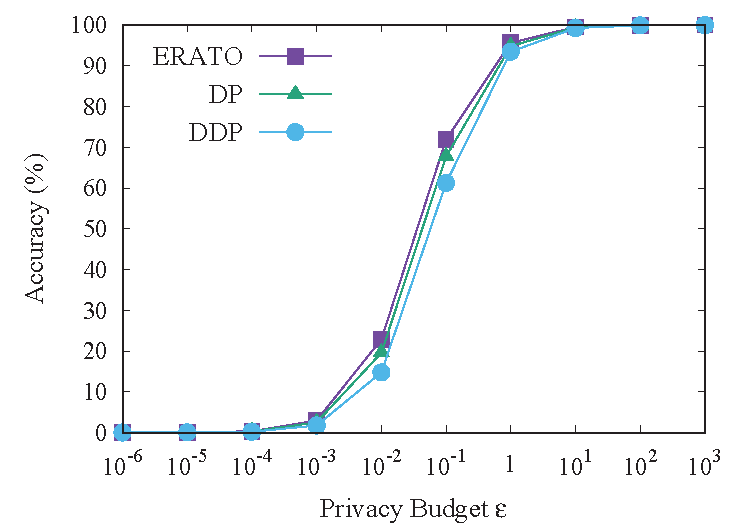
\includegraphics[width=0.31\colwidth]{.//images//WeightAccuracyPercent-ACM.pdf}
  		  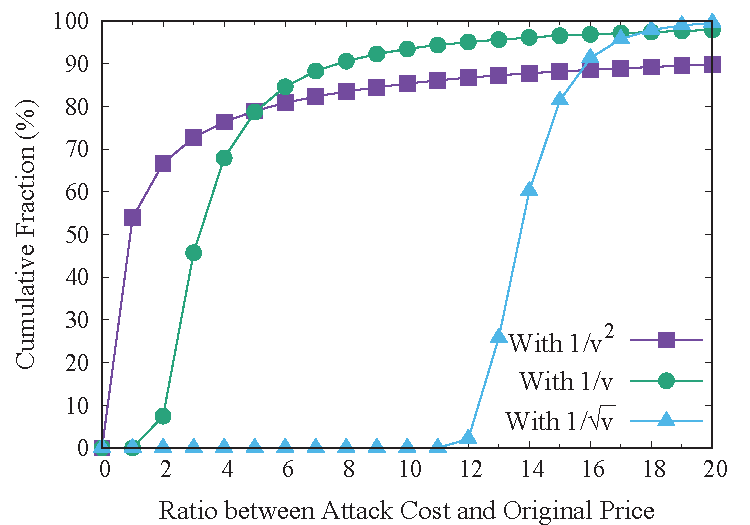
\includegraphics[width=0.31\colwidth]{.//images//Variance-ACM.pdf}
  		  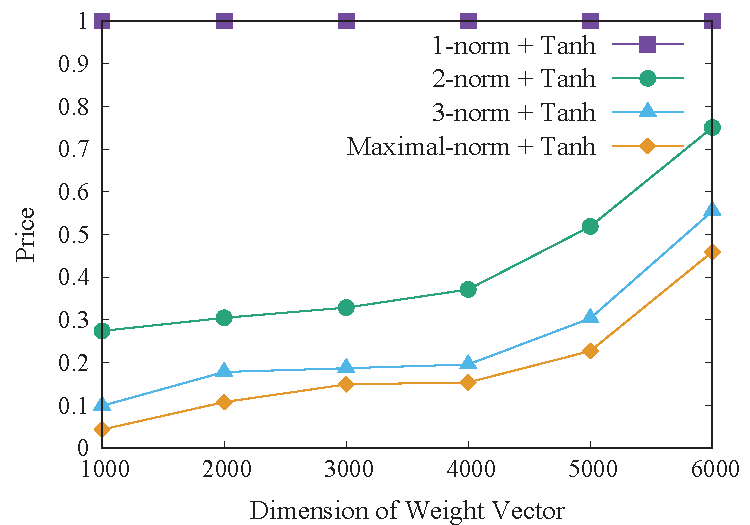
\includegraphics[width=0.31\colwidth]{.//images//WeightDimensions-ACM.pdf}
  	  \end{tikzfigure}

      \coloredbox
      {
          Fig.~\ref{fig:sp:weighted:sum} reveals that ERATO can balance privacy and utility better than differential privacy (DP) and dependent differential privacy (DDP), and avoid arbitrage in service pricing.
      }
     \begin{tikzfigure}[DP and ERATO based Privacy Compensations in Weighted Sum. ]
  	     \label{fig:pc:weighted:sum}
  		  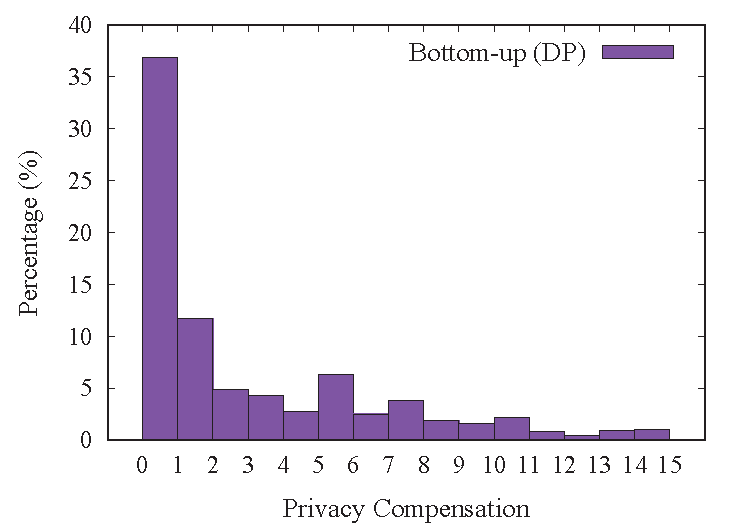
\includegraphics[width=0.232\colwidth]{.//images//HisWeight//HistWeight-BU-DP-ACM.pdf}
  		  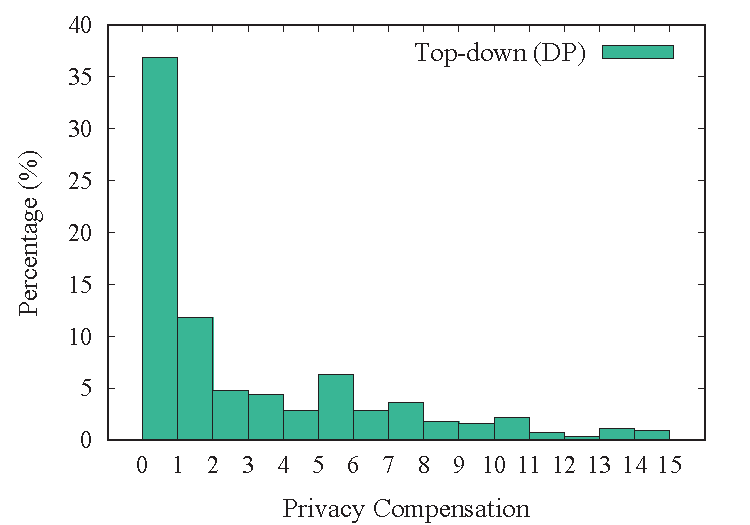
\includegraphics[width=0.232\colwidth]{.//images//HisWeight//HistWeight-TD-DP-ACM.pdf}
  		  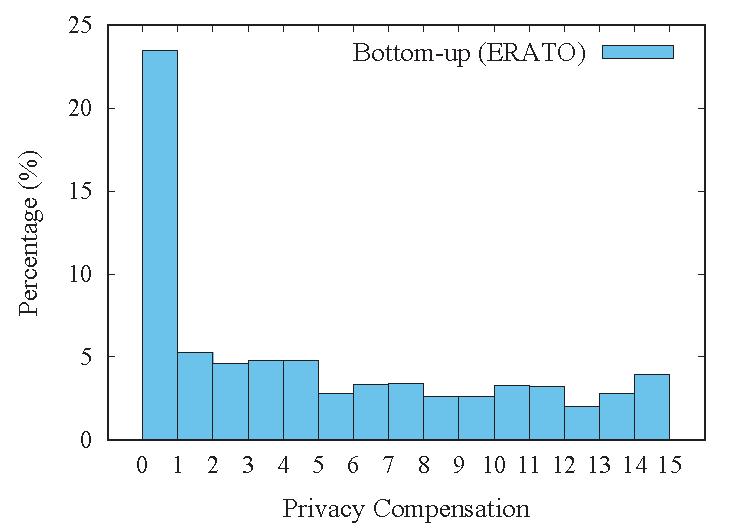
\includegraphics[width=0.232\colwidth]{.//images//HisWeight//HistWeight-BU-DDP-ACM.pdf}
  		  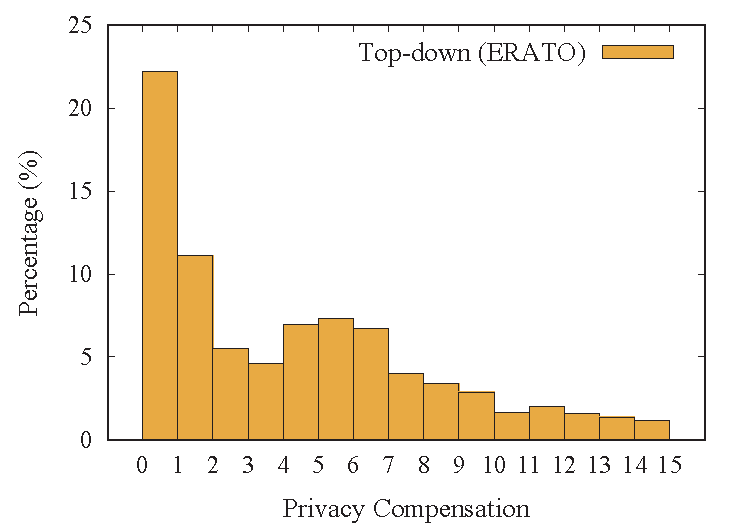
\includegraphics[width=0.232\colwidth]{.//images//HisWeight//HistWeight-TD-DDP-ACM.pdf}
     \end{tikzfigure}
     \vspace{-.6cm}
     \begin{tikzfigure}[ERATO based Privacy Compensation in Gaussian Distribution Fitting.]
  	     \label{fig:pc:distribution:fitting}
  		  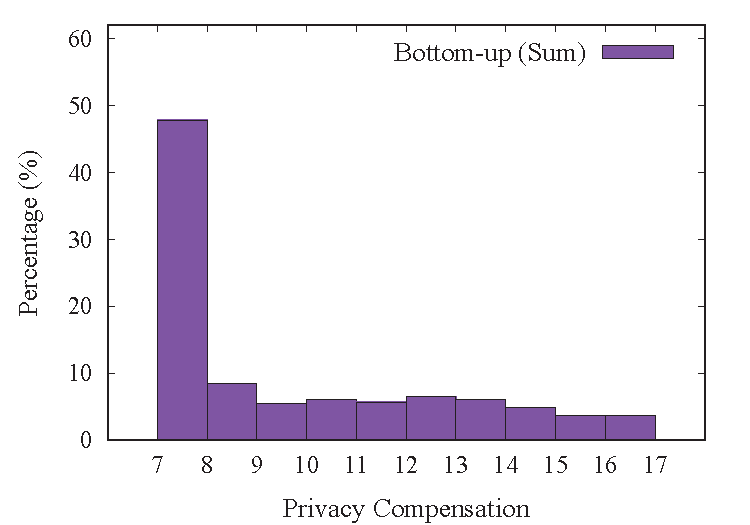
\includegraphics[width=0.232\colwidth]{.//images//HisGaussian//HistGaussian-BU-NEW-ACM.pdf}
  		  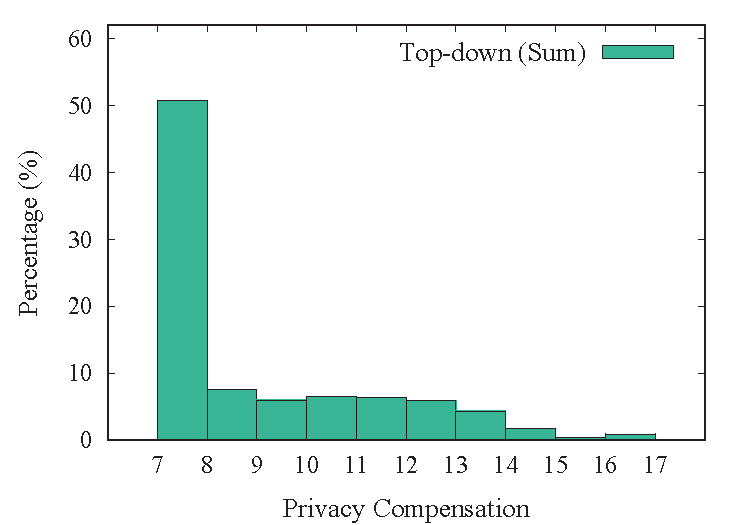
\includegraphics[width=0.232\colwidth]{.//images//HisGaussian//HistGaussian-TD-NEW-ACM.pdf}
  		  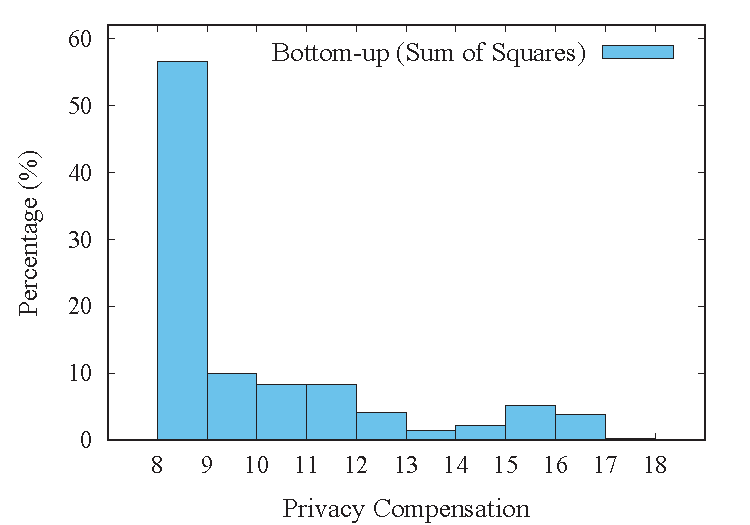
\includegraphics[width=0.232\colwidth]{.//images//HisGaussian//HistGaussian-BU-SQ-NEW-ACM.pdf}
  		  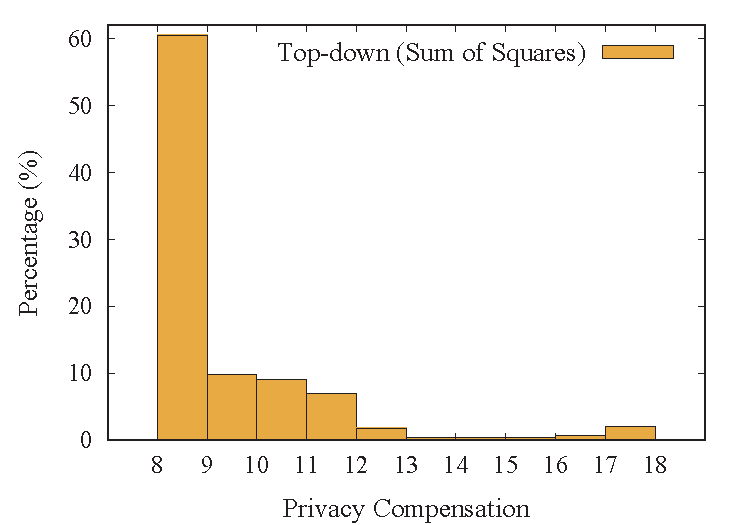
\includegraphics[width=0.232\colwidth]{.//images//HisGaussian//HistGaussian-TD-SQ-NEW-ACM.pdf}
     \end{tikzfigure}
     \vspace{-.6cm}
     \begin{tikzfigure}[ERATO based Privacy Compensation in Twitter/Google+ Degree Distribution. ]
  	      \label{fig:pc:degree:distribution}
  		  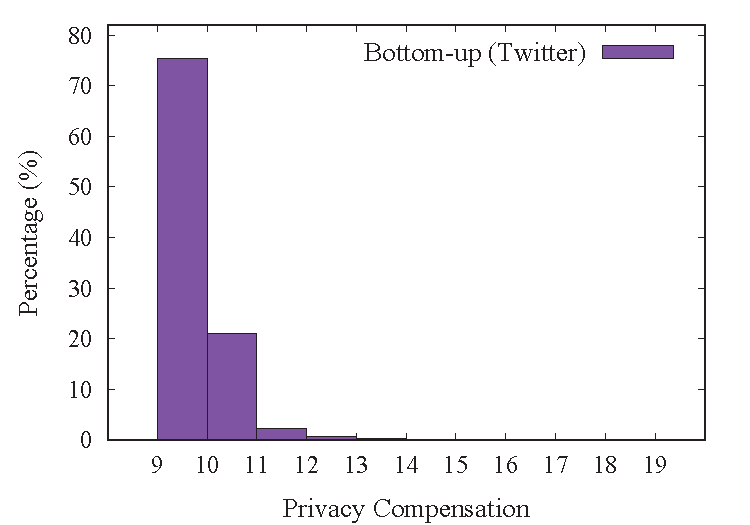
\includegraphics[width=0.232\colwidth]{.//images//HisTwitter//HisDegree-TWITTER-BU-ACM.pdf}
  		  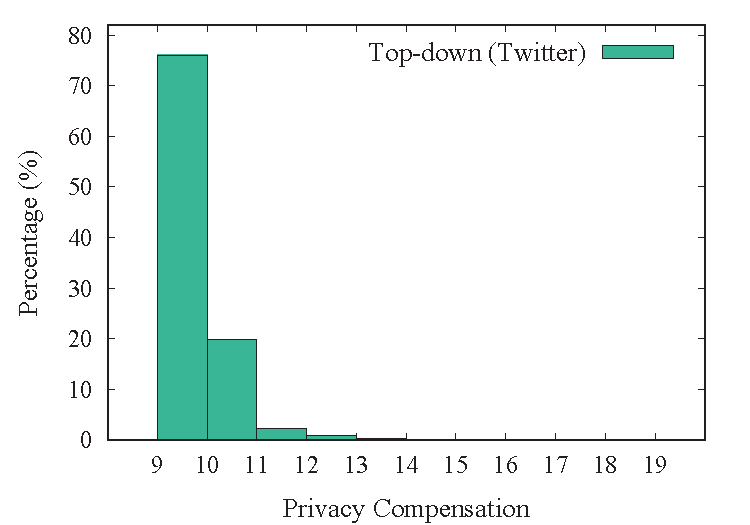
\includegraphics[width=0.232\colwidth]{.//images//HisTwitter//HisDegree-TWITTER-TD-ACM.pdf}
  		  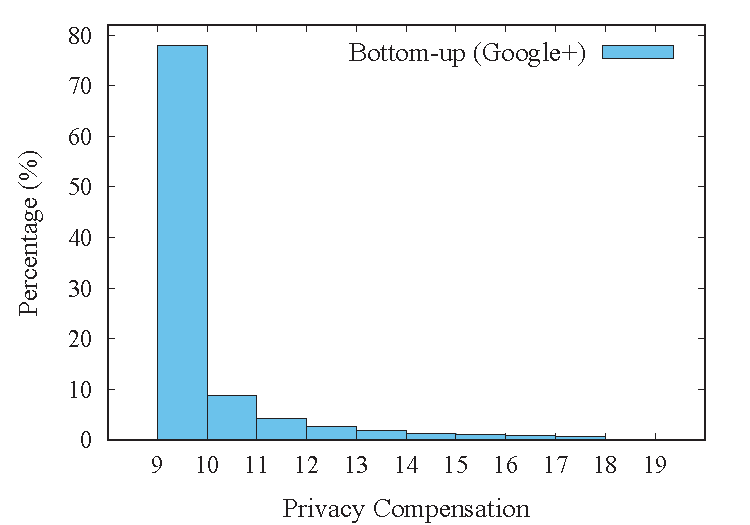
\includegraphics[width=0.232\colwidth]{.//images//HisGoogle//HisDegree-GOOGLE-BU-ACM.pdf}
  		  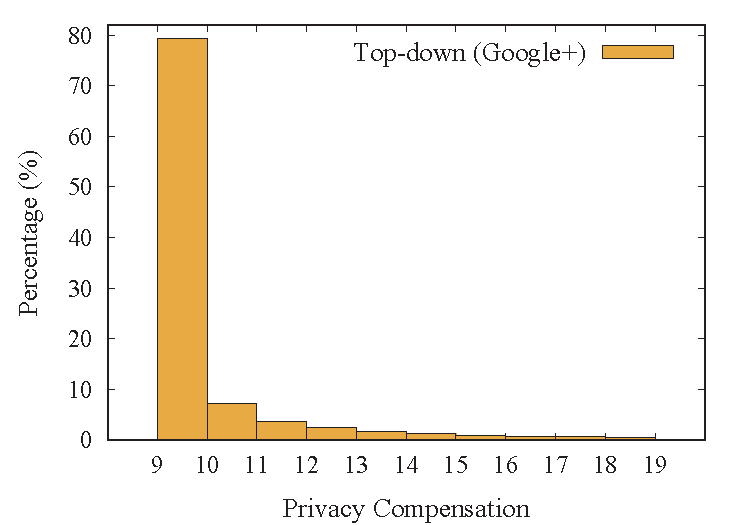
\includegraphics[width=0.232\colwidth]{.//images//HisGoogle//HisDegree-GOOGLE-TD-ACM.pdf}
       \end{tikzfigure}

       \coloredbox
       {
          These figures reveal that in the context of common aggregate statistics, the bottom-up and top-down designs of privacy compensation in ERATO can compensate the data owners for their privacy losses more fairly than DP based approaches.
       }
       \vspace{-.2cm}
   }
   \block{\sc Conclusions}
   {
  	\vspace{-.3cm}
	\begin{itemize}[labelsep=\fontdimen2\font]
      \item Have considered how to trade noisy aggregate statistics over private correlated data  from the perspective of a data broker in data markets, and thus proposed ERATO.
      \item Have applied ERATO to three different aggregate statistics, and extensively evaluate their performances on four real-world datasets.
      \item Evaluation results have demonstrated the feasibility of ERATO, from privacy and utility guarantees, arbitrage-free pricing functions, and fine-grained privacy compensations.
	\end{itemize}
        % \vspace{.1cm}
    \begin{center}
    	
\includegraphics[width=0.7\colwidth]{images/logo.png}
    \end{center}
     \vspace{-.6cm}
  }
\end{columns}
\end{document}